\scanpage{239}

\margin{\unsure{$G_m$}$\longrightarrow$ \quad \unsure{$G_n$}$\longrightarrow$}

\margin{\diagram{\begin{tikzcd}[column sep=large]
\deleted{\unsure{P|R}}\arrow[r] & \deleted{Q}\arrow[r] & \deleted{R}
\end{tikzcd}}}
\margin{\deleted{$\operatorname{Im}\unsure{P}\cap\operatorname{Ker}(\unsure{C|Q})$}}
\margin{\deleted{$\operatorname{Im}(\unsure{P|R}\longrightarrow Q)\cap\operatorname{Ker}(Q\longrightarrow R)$}}

En effet, si $G_{m,n}=\operatorname{Im}(G_m\unsure{\text{---}|\longrightarrow}G_n)$ pour $m\geq n$, on sait que
\[
G_{m,n}(k)\unsure{=|\supset}\operatorname{Im}(G_m(k)\unsure{\text{---}|\longrightarrow}G_n(k))
\]
\unsure{par ce fait que} $\mathrm H^1(k,N_{m,n})=0$. Par suite, \inserted{pour $n$ fixé,} \unsure{la suite|les suites} des $\operatorname{Im}(G_m(k)\unsure{\text{---}|\longrightarrow}G_n(k))$ \unsure{sont|est} \unsure{stationnaires|stationnaire}.

N.B. En car. 0, \unsure{tout} groupe algébrique \unsure{commutatif} unipotent est connexe \inserted{et un gr \uline{vectoriel}}, donc si les $\operatorname{Ker}(G_{n+1}\longrightarrow G_n)$ sont des groupes \deleted{\unsure{vectoriels}}\inserted{unipotents}, \deleted{\unsure{$G_m$} \illegible{3}}\inserted{alors \deleted{et} les} \deleted{\unsure{les}} $\operatorname{Ker}(G_m\longrightarrow G_n)$ pour $m\geq\deleted{\unsure{n_0}}n$ \unsure{sont} des groupes vectoriels, en particulier connexes.

\margin{\unsure{voir ça}}
\figure{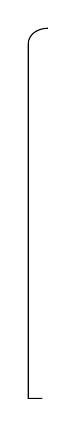
\begin{tikzpicture}[x=1cm,y=1cm]
\draw (0.18,0) -- (0,0) -- (0,4.5) to[out=90,in=180] (0.25,4.7);
\end{tikzpicture}}

\uline{Pr.} Soit $\mathfrak X$ un schéma formel \inserted{\figure{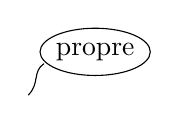
\begin{tikzpicture}[baseline=-.5ex]\draw (0,0) ellipse (.7 and .3);\node at (0,0) {propre};\draw (-.65,-.15)..controls(-.8,-.25)and(-.7,-.4)..(-.85,-.55);\end{tikzpicture}}} sur un anneau local noethérien complet $A$, contenant un \uline{corps $k$ de car. 0} tel que \deleted{\unsure{le}} $k(A)$ soit fini sur $k$. Considérons les $X_n$ comme des schémas propres sur $k$, \deleted{Alors} considérons le syst. projectif
\[
(\underline{\operatorname{Pic}}_{X_n/k})
\]
Alors ce syst. \unsure{satisfait} aux conditions

\figure{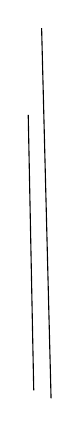
\begin{tikzpicture}[x=1cm,y=1cm]
\draw (0.12,0) -- (0,4.7);
\draw (-0.1,0.1) -- (-0.17,3.6);
\end{tikzpicture}}

\mspage{238}
